\begin{frame}
\begin{center}
Trees That Grow is a programming idiom, described in 2017 by Shayan Najd \& Simon PJ\cite{najd2016trees}

\noindent\makebox[\linewidth]{\rule{\paperwidth}{0.4pt}}

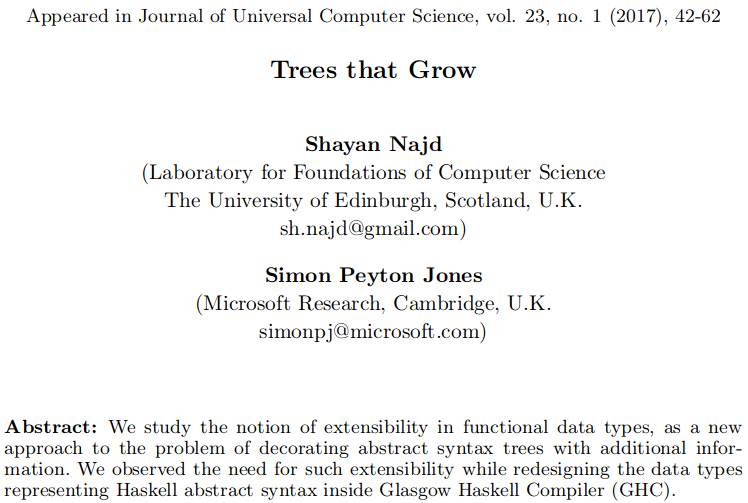
\includegraphics[height=0.5\textheight]{image/ttg-paper.png}
\end{center}
\end{frame}

\begin{frame}
\begin{center}
Problem

>=3 similar data types for Haskell source

\begin{itemize}
\item GHC data type \lstinline{HsSyn}
\item \lstinline{TH.Syntax} data type for Template Haskell
\item libraries such as \lstinline{haskell-src-ext}
\end{itemize}
\end{center}
\end{frame}

\begin{frame}
\begin{center}
How to keep them all in sync?

How to program against them in general?
\end{center}
\end{frame}

